\documentclass[8pt,a4paper,compress]{beamer}

\usepackage{/home/siyer/lib/slides}

\title{Designing Data Types}
\date{}

\begin{document}
\begin{frame}
\vfill
\titlepage
\end{frame}

\begin{frame}
\frametitle{Outline}
\tableofcontents
\end{frame}

\section{APIs}
\begin{frame}[fragile]
\pause

Precisely specifying a data type using an API improves design because it leads to client code that can clearly express its computation 

\pause
\bigskip

By using APIs to separate clients from implementations, we reap the benefits of standard interfaces for every program that we compose

\pause
\bigskip

APIs should provide to clients just the methods they need and no others
\end{frame}

\section{Encapsulation}
\begin{frame}[fragile]
\pause

The process of separating clients from implementations by hiding information is known as encapsulation

\pause
\bigskip

Encapsulation allows one implementation of an API to be substituted for another

\pause
\bigskip

Encapsulation helps programmers ensure that their code operates as intended

\pause
\bigskip

Python does not enforce encapsulation; instead, through a naming convention, clients are informed that they should not directly access the instance variable, method, or function thus named

\pause
\bigskip

The API should be the only point of dependence between client and implementation --- this is called modular programming
\end{frame}

\section{Immutability}
\begin{frame}[fragile]
\pause

An object from a data type is immutable if its data-type value cannot change once created

\pause
\bigskip

The purpose of many data types (eg, \lstinline{Stopwatch}) is to encapsulate values that do not change, while for many other data types (eg, \lstinline{Turtle}), the very purpose of the abstraction is to encapsulate values as they change 

\pause
\bigskip

Generally, immutable data types are easier to use and harder to misuse because the scope of code that can change object values is far smaller than for mutable types

\pause
\bigskip

In Python, lists are mutable, whereas and strings and tuples are immutable

\pause
\bigskip

The downside of immutability is that we must create a new object for every value, which is called defensive copy

\begin{lstlisting}[language=Python]
class Vector:
    def __init__(self, a):
        self._coords = a[:] # self._coords is a defensive copy of a
        self._n = len(a)
\end{lstlisting}
\end{frame}

\section{Polymorphism}
\begin{frame}[fragile]
\pause

A method (or function) that can take arguments with different types is said to be polymorphic

\pause
\bigskip

Duck typing is a programming style in which the language does not formally specify the requirements for a function's arguments

\pause
\bigskip

Python uses duck typing for all operations (function calls, method calls, and operators), and raises a \lstinline{TypeError} at run time if an operation cannot be applied to an object because it is of an inappropriate type

\pause
\bigskip

Duck typing leads to simpler and more flexible client code and puts the focus on operations rather than the type

\pause
\bigskip

A disadvantage of duck typing is that it is difficult to know precisely what the contract is between the client and the implementation --- the API simply does not carry this information
\end{frame}

\section{Overloading}
\begin{frame}[fragile]
\pause

The ability to define a data type that provides its own definitions of operators is a form of polymorphism known as operator overloading

\pause
\bigskip

In Python, we can overload almost every operator, including operators for arithmetic, comparisons, indexing, and slicing

\pause
\bigskip

We can also overload built-in functions, including absolute value, length, hashing, and type conversion

\pause
\bigskip

Overloading operators and built-in functions makes user-defined types behave more like built-in types

\pause
\bigskip

To perform an operation, Python internally converts the expression into a call on the corresponding special method

\pause
\bigskip

To call a built-in function, Python internally calls the corresponding special method instead

\pause
\bigskip

To overload an operator or built-in function, we include an implementation of the corresponding special method with our own code
\end{frame}

\begin{frame}[fragile]
\pause

Special methods for arithmetic operators
\begin{center}
\begin{tabular}{ccc}
client operation & special method & description \\ \hline
\lstinline$x + y$ & \lstinline$__add__(self, y)$ & sum of $x$ and $y$ \\
\lstinline$x - y$ & \lstinline$__sub__(self, y)$ & difference of $x$ and $y$ \\
\lstinline$x * y$ & \lstinline$__mul__(self, y)$ & product of $x$ and $y$ \\
\lstinline$x ** y$ & \lstinline$__pow__(self, y)$ & $x$ to the power $y$ \\
\lstinline$x / y$ & \lstinline$__div__(self, y)$ & quotient of $x$ and $y$ \\
\lstinline$x // y$ & \lstinline$__floordiv__(self, y)$ & floored quotient of $x$ and $y$ \\
\lstinline$x % y$ & \lstinline$__mod__(self, y)$ & remainder when dividing $x$ by $y$ \\
\lstinline$+x$ & \lstinline$__pos__(self)$ & $x$ \\
\lstinline$-x$ & \lstinline$__neg__(self)$ & arithmetic negation of $x$
\end{tabular} 
\end{center}

\pause
\bigskip

Special methods for comparison operators
\begin{center}
\begin{tabular}{ccc}
client operation & special method & description \\ \hline
\lstinline$x == y$ & \lstinline$__eq__(self, y)$ & are $x$ and $y$ equal? \\
\lstinline$x != y$ & \lstinline$__ne__(self, y)$ & are $x$ and $y$ not equal? \\
\lstinline$x < y$ & \lstinline$__lt__(self, y)$ & is $x$ less than $y$? \\
\lstinline$x <= y$ & \lstinline$__le__(self, y)$ & is $x$ less than or equal to $y$? \\
\lstinline$x > y$ & \lstinline$__gt__(self, y)$ & is $x$ greater than $y$? \\
\lstinline$x >= y$ & \lstinline$__ge__(self, y)$ & is $x$ greater than or equal to $y$?
\end{tabular} 
\end{center}
\end{frame}

\begin{frame}[fragile]
\pause

Special methods for built-in functions
\begin{center}
\begin{tabular}{ccc}
client operation & special method & description \\ \hline
\lstinline$len(x)$ & \lstinline$__len__(self)$ & length of $x$ \\
\lstinline$float(x)$ & \lstinline$__float__(self)$ & float equivalent of $x$ \\
\lstinline$int(x)$ & \lstinline$__int__(self)$ & integer equivalent of $x$ \\
\lstinline$str(x)$ & \lstinline$__str__(self)$ & string representation of $x$ \\
\lstinline$abs(x)$ & \lstinline$__abs__(self)$ & absolute value of $x$ \\
\lstinline$hash(x)$ & \lstinline$__hash__(self)$ & integer hash code for $x$ \\
\lstinline$iter(x)$ & \lstinline$__iter__(self)$ & iterator for $x$
\end{tabular} 
\end{center}
\end{frame}

\section{Functions are Objects}
\begin{frame}[fragile]
\pause

In Python, everything is an object, including functions, which means we can use them as arguments to functions and return them as results

\pause
\bigskip

Defining higher-order functions that manipulate other functions is common both in mathematics and scientific computing

\pause
\bigskip

For example, the following function evaluates the Riemann integral (ie, the area under the curve) of a real-valued function $f()$ in the interval $(a, b)$, using the rectangle rule with $n$ rectangles

\begin{lstlisting}[language=Python]
def integrate(f, a, b, n = 1000):
    total = 0.0
    dt = 1.0 * (b - a) / n
    for i in range(n):
        total += dt * f(a + (i + 0.5) * dt)
    return total
\end{lstlisting}

\pause
\bigskip

The following statement uses the above function to compute the area under the curve $f(x)=x^2$ in the interval $(0, 1)$

\begin{lstlisting}[language=Python]
area = integrate(lambda x : x * x, 0, 1)
\end{lstlisting}
\end{frame}

\section{Examples}
\begin{frame}[fragile]
\pause

A data type \lstinline{Complex} for complex numbers
\begin{center}
\begin{tabular}{cc}
method & description \\ \hline
\lstinline$Complex(x, y)$ & a new complex object $c$ with value $x + yi$ \\
\lstinline$c.re()$ & real part of $c$ \\
\lstinline$c.im()$ & imaginary part of $c$ \\
\lstinline$c.conjugate()$ & conjugate of $c$ \\
\lstinline$c + d$ & sum of $c$ and $d$ \\
\lstinline$c * d$ & product of $c$ and $d$ \\
\lstinline$abs(c)$ & magnitude of $c$ \\
\lstinline$str(c)$ & string representation of $c$
\end{tabular} 
\end{center}

\pause
\bigskip

\begin{minipage}{200pt}
A complex number $z$ in the polar form is expressed as $z = re^{i\theta}$

\bigskip

Polar to cartesian: $x = r\cos \theta$ and $y = r\sin \theta$

\bigskip

Cartesian to polar: $r = \sqrt{x^2 + y^2}$ and $\theta = \arctan(y/x)$

\bigskip

If $z_1 = r_1e^{i\theta_1}$ and $z_2 = r_2e^{i\theta_2}$, then $z_1 z_2 = r_1 r_2 e^{i(\theta_1 + \theta_2)}$
\end{minipage}%
\hfill
\begin{minipage}{100pt}
\begin{center}
\visible<3->{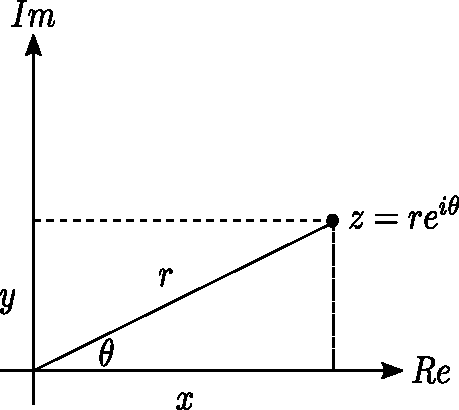
\includegraphics[scale=0.4]{figures/complex_plane_polar.pdf}}
\end{center}
\end{minipage}%
\end{frame}

\begin{frame}[fragile]
\pause

\begin{framed}
\tiny \lstinline{complexpolar.py}: \lstinline{Complex} data type redux. 
\end{framed}

\begin{lstlisting}[language=Python]
import math
import stdio

class Complex:
    def __init__(self, re = 0.0, im = 0.0):
        self._r = math.sqrt(re * re + im * im)
        self._theta = math.atan2(im, re)

    def re(self):
        return self._r * math.cos(self._theta)

    def im(self):
        return self._r * math.sin(self._theta)

    def conjugate(self):
        return Complex(self.re(), -self.im())

    def __add__(self, other):
        re = self.re() + other.re()
        im = self.im() + other.im()
        return Complex(re, im)

    def __mul__(self, other):
        c = Complex(0, 0)
        c._r = self._r * other._r
        c._theta = self._theta + other._theta
        return c
\end{lstlisting}
\end{frame}

\begin{frame}[fragile]
\pause

\begin{lstlisting}[language=Python]
    def __abs__(self):
        return self._r

    def __str__(self):
        return str(self.re()) + ' + ' + str(self.im()) + 'i'

def _main():
    z0 = Complex(1.0, 1.0)
    z = z0
    z = z * z + z0
    z = z * z + z0
    stdio.writeln(z)

if __name__ == '__main__':
    _main()
\end{lstlisting}

\pause

\begin{lstlisting}[language={}]
$ python complexpolar.py 
-7.0 + 7.0i
\end{lstlisting}
\end{frame}

\begin{frame}[fragile]
\pause

A data type \lstinline{Counter} for counting
\begin{center}
\begin{tabular}{cc}
method & description \\ \hline
\lstinline$Counter(id, maxCount)$ & a new counter $c$ named $id$, with maximum value $maxCount$ \\
\lstinline$c.increment()$ & increment $c$, unless its value is $maxCount$ \\
\lstinline$c.value()$ & value of $c$ \\
\lstinline$str(c)$ & string representation of $c$ \\
\lstinline$c == d$ & are $c$ and $d$ equal? \\
\lstinline$c != d$ & are $c$ and $d$ not equal? \\
\lstinline$c < d$ & is $c$ less than $d$? \\
\lstinline$c > d$ & is $c$ greater than $d$? \\
\lstinline$c <= d$ & is $c$ less than or equal to $d$? \\
\lstinline$c >= d$ & is $c$ greater than or equal to $d$? \\
\end{tabular} 
\end{center}
\end{frame}

\begin{frame}[fragile]
\pause

\begin{framed}
\tiny counter.py: Definition of \lstinline{Counter} data type.
\end{framed}

\begin{lstlisting}[language=Python]
import stdio
import stdrandom
import sys

class Counter:
    def __init__(self, id, maxCount):
        self._name = id
        self._maxCount = maxCount
        self._count = 0

    def increment(self):
        if self._count < self._maxCount:
            self._count += 1

    def value(self):
        return self._count

    def __str__(self):
        return self._name + ': ' + str(self._count)

    def __eq__(self, other):
        return self._count == other._count

    def __ne__(self, other):
        return self._count != other._count

    def __lt__(self, other):
        return self._count < other._count
\end{lstlisting}
\end{frame}

\begin{frame}[fragile]
\pause

\begin{lstlisting}[language=Python]
    def __gt__(self, other):
        return self._count > other._count

    def __le__(self, other):
        return self._count <= other._count

    def __ge__(self, other):
        return self._count >= other._count

def _main():
    n = int(sys.argv[1])
    p = float(sys.argv[2])
    heads = Counter('Heads', n)
    tails = Counter('Tails', n)
    for i in range(n):
        if stdrandom.bernoulli(p):
            heads.increment()
        else:
            tails.increment()
    stdio.writeln(heads)
    stdio.writeln(tails)

if __name__ == '__main__':
    _main()
\end{lstlisting}

\pause

\begin{lstlisting}[language={}]
$ python counter.py 1000 .5
Heads: 483
Tails: 517
$ python counter.py 1000 .5
Heads: 503
Tails: 497
$ python counter.py 1000 .3
Heads: 280
Tails: 720
\end{lstlisting}
\end{frame}

\begin{frame}[fragile]
\pause

\begin{minipage}{200pt}
A spatial vector is an abstract entity that has a magnitude and a direction
\end{minipage}%
\hfill
\begin{minipage}{100pt}
\begin{center}
\visible<2->{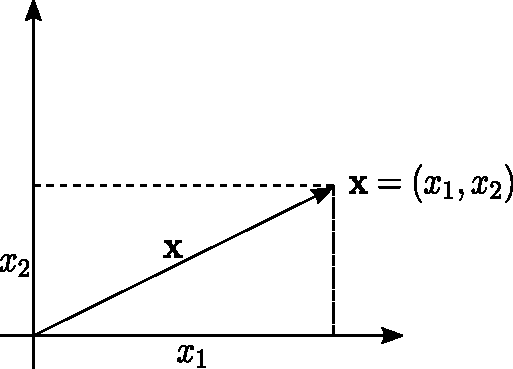
\includegraphics[scale=0.4]{figures/vector.pdf}}
\end{center}
\end{minipage}%

\pause
\bigskip

Vector operations, assuming $\mathbf{x}=(x_1,x_2,\dots,x_n)$, $\mathbf{y}=(y_1,y_2,\dots,y_n)$, and $\alpha \in \mathbb{R}$
\begin{itemize}
\item Addition: $\mathbf{x}+\mathbf{y}=(x_1+y_1,x_2+y_2,\dots,x_n+y_n)$
\item Subtraction: $\mathbf{x}-\mathbf{y}=(x_1-y_1,x_2-y_2,\dots,x_n-y_n)$
\item Scalar product: $\alpha\mathbf{x}=(\alpha x_1,\alpha x_2,\dots,\alpha x_n)$
\item Dot product: $\mathbf{x}\cdot\mathbf{y}=x_1y_1+x_2y_2+\dots+x_ny_n$
\item Magnitude: $|\mathbf{x}|=(x_1^2+x_2^2+\dots+x_n^2)^{1/2}$
\item Direction: $\mathbf{x}/|\mathbf{x}|=(x_1/|\mathbf{x}|,x_2/|\mathbf{x}|,\dots,x_n/|\mathbf{x}|)$
\end{itemize}
\end{frame}

\begin{frame}[fragile]
\pause

A data type \lstinline{Vector} for spatial vectors
\begin{center}
\begin{tabular}{cc}
method & description \\ \hline
\lstinline$Vector(a)$ & a new vector $v$ with Cartesian coordinates taken from the list $a$ \\
\lstinline$v[i]$ & $i$th Cartesian coordinates of $v$ \\
\lstinline$v + w$ & sum of $v$ and $w$ \\
\lstinline$v - w$ & difference of $v$ and $w$ \\
\lstinline$v.scale(alpha)$ & scalar product of float $\alpha$ and $v$ \\
\lstinline$v.dot(w)$ & dot product of $v$ and $w$ \\
\lstinline$v.direction()$ & unit vector in the same direction as $v$ \\
\lstinline$abs(v)$ & magnitude of $v$ \\
\lstinline$len(v)$ & length of $v$ \\
\lstinline$str(v)$ & string representation of $v$
\end{tabular} 
\end{center}
\end{frame}

\begin{frame}[fragile]
\pause

\begin{framed}
\tiny vector.py: Definition of \lstinline{Vector} data type.
\end{framed}

\begin{lstlisting}[language=Python]
import math
import stdarray
import stdio

class Vector:
    def __init__(self, a):
        self._coords = a[:]
        self._n = len(a)

    def __getitem__(self, i):
        return self._coords[i]

    def __add__(self, other):
        result = stdarray.create1D(self._n, 0)
        for i in range(self._n):
            result[i] = self._coords[i] + other._coords[i]
        return Vector(result)

    def __sub__(self, other):
        result = stdarray.create1D(self._n, 0)
        for i in range(self._n):
            result[i] = self._coords[i] - other._coords[i]
        return Vector(result)

    def scale(self, alpha):
        result = stdarray.create1D(self._n, 0)
        for i in range(self._n):
            result[i] = alpha * self._coords[i]
        return Vector(result)
\end{lstlisting}
\end{frame}

\begin{frame}[fragile]
\pause

\begin{lstlisting}[language=Python]
    def dot(self, other):
        result = 0
        for i in range(self._n):
            result += self._coords[i] * other._coords[i]
        return result

    def direction(self):
        return self.scale(1.0 / abs(self))
     
    def __abs__(self):
        return math.sqrt(self.dot(self))

    def __len__(self):
        return self._n

    def __str__(self):
        return str(self._coords)
        
def _main():
    xCoords = [1.0, 2.0, 3.0, 4.0]
    yCoords = [5.0, 2.0, 4.0, 1.0]
    x = Vector(xCoords)
    y = Vector(yCoords)
    stdio.writeln('x        = ' + str(x))
    stdio.writeln('y        = ' + str(y))
    stdio.writeln('x + y    = ' + str(x + y))
    stdio.writeln('10x      = ' + str(x.scale(10.0)))
    stdio.writeln('|x|      = ' + str(abs(x)))
    stdio.writeln('<x, y>   = ' + str(x.dot(y)))
    stdio.writeln('|x - y|  = ' + str(abs(x - y)))

if __name__ == '__main__':
    _main()
\end{lstlisting}
\end{frame}

\begin{frame}[fragile]
\pause

\begin{lstlisting}[language={}]
$ python vector.py
x        = [1.0, 2.0, 3.0, 4.0]
y        = [5.0, 2.0, 4.0, 1.0]
x + y    = [6.0, 4.0, 7.0, 5.0]
10x      = [10.0, 20.0, 30.0, 40.0]
|x|      = 5.47722557505
<x, y>   = 25.0
|x - y|  = 5.09901951359
\end{lstlisting}
\end{frame}

\begin{frame}[fragile]
\pause

A data type \lstinline{Sketch} for compactly representing the content of a document
\begin{center}
\begin{tabular}{cc}
method & description \\ \hline
\lstinline$Sketch(text, k, d)$ & \makecell{a new sketch $s$ built from the string $text$ \\ using $k$-grams and dimension $d$} \\
\lstinline$s.similarTo(t)$ & \makecell{similarity measure between sketches $s$ and $t$ (a float \\ between 0.0 and 1.0)} \\
\lstinline$str(s)$ & string representation of $s$
\end{tabular} 
\end{center}
\end{frame}

\begin{frame}[fragile]
\pause

\begin{framed}
\tiny sketch.py: Definition of \lstinline{Sketch} data type. 
\end{framed}

\begin{lstlisting}[language=Python]
import stdarray
import stdio
import sys
from vector import Vector

class Sketch:
    def __init__(self, text, k, d):
        freq = stdarray.create1D(d, 0)
        for i in range(len(text) - k):
            kgram = text[i:i + k]
            h = hash(kgram)
            freq[h % d] += 1
        vector = Vector(freq)
        self._sketch = vector.direction()

    def similarTo(self, other):
        return self._sketch.dot(other._sketch)

    def __str__(self):
        return str(self._sketch)

def _main():
    text = stdio.readAll()
    k = int(sys.argv[1])
    d = int(sys.argv[2])
    sketch = Sketch(text, k, d)
    stdio.writeln(sketch)

if __name__ == '__main__':
    _main()
\end{lstlisting}
\end{frame}

\begin{frame}[fragile]
\pause

\begin{lstlisting}[language={}]
$ more genome20.txt
ATAGATGCATAGCGCATAGC
\end{lstlisting}

\pause

\begin{lstlisting}[language={}]
$ python sketch.py 2 16 < genome20.txt 
[0.37210420376762543, 0.37210420376762543, 0.49613893835683387, 0.0, 
0.12403473458920847, 0.0, 0.0, 0.0, 0.0, 0.0, 0.24806946917841693, 0.0, 
0.12403473458920847, 0.6201736729460423, 0.0, 0.0]
\end{lstlisting}
\end{frame}

\begin{frame}[fragile]
\pause

\begin{framed}
\tiny comparedocuments.py: Accept integers $k$ and $d$ as command-line arguments, read a document list from standard input, compute $d$-dimensional profiles based on $k$-gram frequencies for all the documents, and write a matrix of similarity measures between all pairs of documents.
\end{framed}

\begin{lstlisting}[language=Python]
import stdarray
import stdio
import sys
from instream import InStream
from sketch import Sketch

def main():
    k = int(sys.argv[1])
    d = int(sys.argv[2])
    filenames = stdio.readAllStrings()
    sketches = stdarray.create1D(len(filenames))
    for i in range(len(filenames)):
        text = InStream(filenames[i]).readAll()
        sketches[i] = Sketch(text, k, d)
    stdio.write('    ')
    for i in range(len(filenames)):
        stdio.writef('%8.4s', filenames[i])
    stdio.writeln()
    for i in range(len(filenames)):
        stdio.writef('%.4s', filenames[i])
        for j in range(len(filenames)):
            stdio.writef('%8.2f', sketches[i].similarTo(sketches[j]))
        stdio.writeln()
    
if __name__ == '__main__':
    main()
\end{lstlisting}
\end{frame}

\begin{frame}[fragile]
\pause

\begin{lstlisting}[language={}]
$ more documents.txt
constitution.txt
tomsawyer.txt
huckfinn.txt
prejudice.txt
vector.py
djia.csv
amazon.html
actg.txt
\end{lstlisting}

\pause

\begin{lstlisting}[language={}]
$ python comparedocuments.py 5 10000 < documents.txt
        cons    toms    huck    prej    vect    djia    amaz    actg
cons    1.00    0.67    0.61    0.64    0.10    0.18    0.19    0.12
toms    0.67    1.00    0.93    0.87    0.08    0.23    0.19    0.15
huck    0.61    0.93    1.00    0.81    0.06    0.21    0.15    0.14
prej    0.64    0.87    0.81    1.00    0.07    0.25    0.19    0.16
vect    0.10    0.08    0.06    0.07    1.00    0.03    0.17    0.01
djia    0.18    0.23    0.21    0.25    0.03    1.00    0.13    0.12
amaz    0.19    0.19    0.15    0.19    0.17    0.13    1.00    0.09
actg    0.12    0.15    0.14    0.16    0.01    0.12    0.09    1.00
\end{lstlisting}
\end{frame}

\begin{frame}[fragile]
\pause

A comparable data type \lstinline{Planet} for representing planets
\begin{center}
\begin{tabular}{cc}
method & description \\ \hline
\lstinline$Planet(name, moons)$ & create a new planet $p$ given its name and number of moons \\
\lstinline$cmp(p, q)$ & \makecell{compare planets $p$ and $q$ by name (return negative integer, zero, \\ or positive integer depending on whether the name of $p$ is less \\ than, equal to, or greater than the name of $q$)} \\
\lstinline$str(p)$ & string representation of $p$
\end{tabular} 
\end{center}
\end{frame}

\begin{frame}[fragile]
\pause

\begin{framed}
\tiny planet.py: Definition of \lstinline{Planet} data type.
\end{framed}

\begin{lstlisting}[language=Python]
import stdio

class Planet:
    def __init__(self, name, moons):
        self._name = name
        self._moons = moons

    def __cmp__(self, other):
        return cmp(self._name, other._name)
        
    def __str__(self):
        return self._name + ", " + str(self._moons)
\end{lstlisting}
\end{frame}

\begin{frame}[fragile]
\pause

\begin{lstlisting}[language=Python]
def _main():
    planets = [None] * 8
    planets[0] = Planet("Mercury", 0)
    planets[1] = Planet("Venus", 0)
    planets[2] = Planet("Earth", 1)
    planets[3] = Planet("Mars", 2)
    planets[4] = Planet("Jupiter", 67)
    planets[5] = Planet("Saturn", 62)
    planets[6] = Planet("Uranus", 27)
    planets[7] = Planet("Neptune", 14)
    stdio.writeln("Unsorted:")
    for v in planets:
        stdio.writeln("  " + str(v))
    planets.sort()
    stdio.writeln("Sorted by name:")
    for v in planets:
        stdio.writeln("  " + str(v))
    planets.sort(cmp = lambda x, y: cmp(x._moons, y._moons))
    stdio.writeln("Sorted by # of moons:")
    for v in planets:
        stdio.writeln("  " + str(v))

if __name__ == '__main__':
    _main()
\end{lstlisting}
\end{frame}

\begin{frame}[fragile]
\pause

\begin{lstlisting}[language={}]
$ python planet.py 
Unsorted:
  Mercury, 0
  Venus, 0
  Earth, 1
  Mars, 2
  Jupiter, 67
  Saturn, 62
  Uranus, 27
  Neptune, 14
Sorted by name:
  Earth, 1
  Jupiter, 67
  Mars, 2
  Mercury, 0
  Neptune, 14
  Saturn, 62
  Uranus, 27
  Venus, 0
Sorted by # of moons:
  Mercury, 0
  Venus, 0
  Earth, 1
  Mars, 2
  Neptune, 14
  Uranus, 27
  Saturn, 62
  Jupiter, 67
\end{lstlisting}
\end{frame}

\begin{frame}[fragile]
\pause

An iterable \lstinline{Fibonacci} data type for iterating over Fibonacci sequences
\begin{center}
\begin{tabular}{cc}
method & description \\ \hline
\lstinline$Fibonacci(n)$ & a new object $f$ for iterating over the first $n$ Fibonacci numbers \\
\lstinline$iter(f)$ & an iterable object $fiter$ on $f$ \\
\lstinline$next(fiter)$ & the next number in the Fibonacci sequence $fiter$
\end{tabular} 
\end{center}
\end{frame}

\begin{frame}[fragile]
\pause

\begin{framed}
\tiny fibonacci.py: Definition of \lstinline{Fibonacci} data type.
\end{framed}

\begin{lstlisting}[language=Python]
import stdio
import sys

class Fibonacci:
    def __init__(self, n):
        self._n = n
        self._current = 0
        self._a = 1
        self._b = 1

    def __iter__(self):
        return self
        
    def next(self):
        self._current += 1
        if self._current > self._n:
            raise StopIteration
        if self._current <= 2:
            return 1
        self._a, self._b = self._b, self._a + self._b
        return self._b

def _main():
    n = int(sys.argv[1])
    for i in Fibonacci(n):
        stdio.writeln(i)

if __name__ == '__main__':
    _main()
\end{lstlisting}
\end{frame}

\begin{frame}[fragile]
\pause

\begin{lstlisting}[language={}]
>>> from fibonacci import Fibonacci
>>> f = Fibonacci(5)
>>> fiter = iter(f) # calls f.__iter__()
>>> next(fiter)     # calls fiter.next()
1
>>> next(fiter)
1
>>> next(fiter)
2
>>> next(fiter)
3
>>> next(fiter)
5
>>> next(fiter)
Traceback (most recent call last):
  File "<stdin>", line 1, in <module>
StopIteration
>>> 
\end{lstlisting}

\pause

\begin{lstlisting}[language={}]
$ python fibonacci.py 10
1
1
2
3
5
8
13
21
34
55
\end{lstlisting}
\end{frame}

\section{Inheritance}
\begin{frame}[fragile]
\pause

Python provides language support for defining relationships among classes, known as inheritance

\pause
\bigskip

Inheritance enables subclassing, where the idea is to define a new class (subclass, or derived class) that inherits instance variables and methods from another class (superclass, or base class)

\begin{lstlisting}[language={}]
class DerivedClassName(BaseClassName):
    <statement>
    <statement>
    ...
\end{lstlisting}

\pause
\bigskip

Every class in Python implicitly inherits from \lstinline{object}

\pause
\bigskip

Python supports two built-in functions that work with inheritance
\begin{itemize}
\item \lstinline{isinstance(o, T)} checks if instance \lstinline{o} is of type \lstinline{T}
\item \lstinline{issubclass(T1, T2)} checks if \lstinline{T1} is a subclass of \lstinline{T2}
\end{itemize}

\pause
\bigskip

Python supports a limited form of multiple inheritance as well

\begin{lstlisting}[language={}]
class DerivedClassName(Base1, Base2, Base3):
    <statement>
    <statement>
    ...
\end{lstlisting}
\end{frame}

\section{Design by Contract}
\begin{frame}[fragile]
\pause

Design by contract model is one in which the designer of a data type expresses
\begin{itemize}
\item A precondition - the condition that the client promises to satisfy when calling a method
\item A postcondition - the condition that the implementation promises to achieve when returning from a method
\item Invariants - any condition that the implementation promises to satisfy while the method is executing 
\item Side effects - any other change in state that the method could cause
\end{itemize}

\pause
\bigskip

Exceptions and assertions are Python language mechanisms that enable us to test these conditions
\end{frame}

\begin{frame}[fragile]
\pause

An exception is a disruptive event that occurs while a program is running, often to signal an error

\pause
\bigskip

The action taken in response is known as raising an exception (or error)

\pause
\bigskip

We can raise our own exceptions as follows
\begin{lstlisting}[language=Python]
raise Exception('Error message here.')
\end{lstlisting} 

\pause
\bigskip

For example, in \lstinline{vector.py}, we can raise an exception in \lstinline{__add__()} if the two \lstinline{Vectors} to be added have different dimensions
\begin{lstlisting}[language=Python]
if len(self) != len(other):
    raise Exception('vectors have different dimensions')
\end{lstlisting} 

\pause
\bigskip

We can handle exceptions using a try-except block

\pause
\bigskip

For example
\begin{lstlisting}[language=Python]
(x, y) = (5, 0)
try:
    z = x / y
except ZeroDivisionError as e:
    z = e
stdio.writeln(z)
\end{lstlisting} 
\end{frame}

\begin{frame}[fragile]
\pause

An assertion is a boolean expression that we affirm is \lstinline{True}, and if it is \lstinline{False}, the program will raise an \lstinline{AssertionError} at run time

\pause
\bigskip

For example, in \lstinline{counter.py}, we might check that the counter is never negative by adding the following assertion as the last statement in \lstinline{increment()}
\begin{lstlisting}[language=Python]
assert self.__count >= 0
\end{lstlisting} 

\pause
\bigskip

We can also include an optional message, such as
\begin{lstlisting}[language=Python]
assert self.__count >= 0, 'Negative count detected'
\end{lstlisting} 
\end{frame}
\end{document}
